\section{Projektowanie tabel, kluczy, kluczy obcych, powiązań między tabelami, indeksów, etc. w oparciu o zdefiniowany diagram ERD;} 

%na tym etapie następuje „sprecyzowanie” struktury bazy danych wraz ze szczegółami technicznymi. Projekt bazy w języku SQL.

%\begin{figure}[!htp]
%    \centering
%    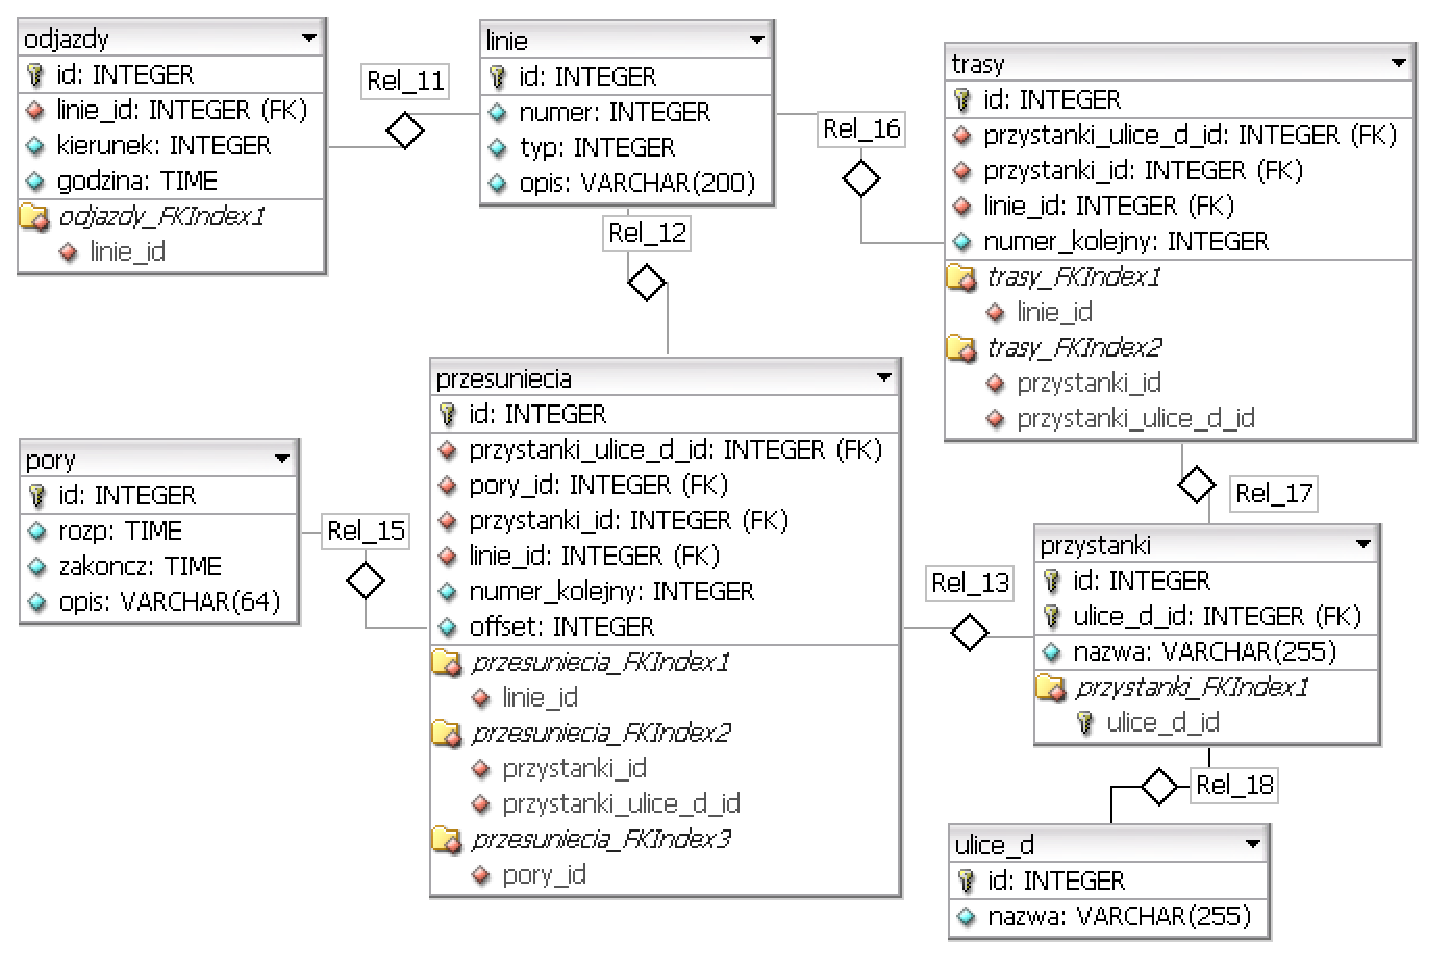
\includegraphics[width=0.75\textwidth]{./img/busag_model.eps}
%    \caption{Tabele}
%    \label{fig:tabs}
%\end{figure}

\begin{lstlisting}
SET client_encoding = 'UTF8';
SET standard_conforming_strings = off;
SET check_function_bodies = false;
SET client_min_messages = warning;
SET escape_string_warning = off;

COMMENT ON SCHEMA public IS 'Standard public schema';


SET search_path = public, pg_catalog;
SET default_tablespace = '';
SET default_with_oids = false;

CREATE TABLE ulice_d (
    id integer NOT NULL,
    nazwa character varying(255) NOT NULL
);

ALTER TABLE public.ulice_d OWNER TO busag;

COMMENT ON TABLE ulice_d IS 'Slownik ulic';
COMMENT ON COLUMN ulice_d.id IS 'Klucz glowny';
COMMENT ON COLUMN ulice_d.nazwa IS 'Nazwa ulicy';

CREATE SEQUENCE dict_ulice_id_seq
    INCREMENT BY 1
    NO MAXVALUE
    NO MINVALUE
    CACHE 1;

ALTER TABLE public.dict_ulice_id_seq OWNER TO busag;

ALTER SEQUENCE dict_ulice_id_seq OWNED BY ulice_d.id;

CREATE TABLE linie (
    numer integer NOT NULL,
    typ smallint DEFAULT 0 NOT NULL,
    opis character varying(200)
);

ALTER TABLE public.linie OWNER TO busag;

CREATE TABLE odjazdy (
    id integer NOT NULL,
    linie_id integer NOT NULL,
    godzina time without time zone DEFAULT '12:00:00'::time without time zone NOT NULL,
    kierunek bit(1) NOT NULL
);

ALTER TABLE public.odjazdy OWNER TO busag;

COMMENT ON TABLE odjazdy IS 'Odjazdy autobusow';
COMMENT ON COLUMN odjazdy.godzina IS 'Godzina odjazdu';

CREATE SEQUENCE odjazdy_id_seq
    INCREMENT BY 1
    NO MAXVALUE
    NO MINVALUE
    CACHE 1;


ALTER TABLE public.odjazdy_id_seq OWNER TO busag;

ALTER SEQUENCE odjazdy_id_seq OWNED BY odjazdy.id;


CREATE TABLE pory (
    id integer NOT NULL,
    rozp time without time zone DEFAULT '12:00:00'::time without time zone NOT NULL,
    zakoncz time without time zone DEFAULT '12:00:00'::time without time zone NOT NULL,
    opis character varying(64) NOT NULL
);

ALTER TABLE public.pory OWNER TO busag;

COMMENT ON TABLE pory IS 'Table por dnia';
COMMENT ON COLUMN pory.id IS 'ID';
COMMENT ON COLUMN pory.rozp IS 'Pora rozpoczecia';
COMMENT ON COLUMN pory.zakoncz IS 'Godzina zakonczenia pory';
COMMENT ON COLUMN pory.opis IS 'Opis';

CREATE SEQUENCE pory_id_seq
    INCREMENT BY 1
    NO MAXVALUE
    NO MINVALUE
    CACHE 1;


ALTER TABLE public.pory_id_seq OWNER TO busag;

ALTER SEQUENCE pory_id_seq OWNED BY pory.id;

CREATE TABLE przesuniecia (
    id integer NOT NULL,
    "offset" interval DEFAULT '00:00:00'::interval NOT NULL,
    trasy_id integer NOT NULL,
    powrotna bit(1) DEFAULT B'0'::"bit" NOT NULL
);

ALTER TABLE public.przesuniecia OWNER TO busag;

COMMENT ON COLUMN przesuniecia.id IS 'Klucz glowny';
COMMENT ON COLUMN przesuniecia.powrotna IS 'Czy trasa jest odwrotna';

CREATE SEQUENCE przesuniecia_id_seq
    INCREMENT BY 1
    NO MAXVALUE
    NO MINVALUE
    CACHE 1;

ALTER TABLE public.przesuniecia_id_seq OWNER TO busag;

ALTER SEQUENCE przesuniecia_id_seq OWNED BY przesuniecia.id;

CREATE TABLE przystanki (
    id integer NOT NULL,
    nazwa character varying(75) NOT NULL,
    ulica1_id integer NOT NULL,
    ulica2_id integer
);

ALTER TABLE public.przystanki OWNER TO busag;

COMMENT ON COLUMN przystanki.ulica1_id IS 'Klucz obcy (opcjonalny) wskazujacy na ulice druga';

CREATE SEQUENCE przystanki_id_seq
    INCREMENT BY 1
    NO MAXVALUE
    NO MINVALUE
    CACHE 1;

ALTER TABLE public.przystanki_id_seq OWNER TO busag;

ALTER SEQUENCE przystanki_id_seq OWNED BY przystanki.id;

CREATE TABLE trasy (
    id integer NOT NULL,
    linie_id integer NOT NULL,
    przystanki_id integer NOT NULL,
    numer_kolejny smallint NOT NULL
);

ALTER TABLE public.trasy OWNER TO busag;

CREATE VIEW timetable_view AS
    SELECT odjazdy.linie_id AS linia_numer, trasy.numer_kolejny, przystanki.id AS przystanek_id, przystanki.nazwa AS przystanek, (przesuniecia."offset" + odjazdy.godzina) AS odj, odjazdy.id AS odj_id, odjazdy.kierunek FROM (((przesuniecia JOIN trasy ON ((przesuniecia.trasy_id = trasy.id))) JOIN przystanki ON ((trasy.przystanki_id = przystanki.id))) JOIN odjazdy ON ((odjazdy.linie_id = trasy.linie_id))) WHERE (odjazdy.kierunek = przesuniecia.powrotna) ORDER BY odjazdy.linie_id, trasy.numer_kolejny;

ALTER TABLE public.timetable_view OWNER TO busag;

CREATE SEQUENCE trasy_id_seq
    INCREMENT BY 1
    NO MAXVALUE
    NO MINVALUE
    CACHE 1;

ALTER TABLE public.trasy_id_seq OWNER TO busag;

ALTER SEQUENCE trasy_id_seq OWNED BY trasy.id;

CREATE VIEW trasy_view AS
    SELECT trasy.przystanki_id, linie.numer, trasy.numer_kolejny, (SELECT przystanki.nazwa FROM przystanki WHERE (przystanki.id = trasy.przystanki_id)) AS nazwa FROM (trasy JOIN linie ON ((linie.numer = trasy.linie_id)));


ALTER TABLE public.trasy_view OWNER TO busag;

ALTER TABLE odjazdy ALTER COLUMN id SET DEFAULT nextval('odjazdy_id_seq'::regclass);

ALTER TABLE pory ALTER COLUMN id SET DEFAULT nextval('pory_id_seq'::regclass);

ALTER TABLE przesuniecia ALTER COLUMN id SET DEFAULT nextval('przesuniecia_id_seq'::regclass);

ALTER TABLE przystanki ALTER COLUMN id SET DEFAULT nextval('przystanki_id_seq'::regclass);

ALTER TABLE trasy ALTER COLUMN id SET DEFAULT nextval('trasy_id_seq'::regclass);

ALTER TABLE ulice_d ALTER COLUMN id SET DEFAULT nextval('dict_ulice_id_seq'::regclass);

ALTER TABLE ONLY ulice_d
    ADD CONSTRAINT dict_ulice_pkey PRIMARY KEY (id);

ALTER TABLE ONLY linie
    ADD CONSTRAINT linie_numer_key UNIQUE (numer);

ALTER TABLE ONLY linie
    ADD CONSTRAINT linie_pkey PRIMARY KEY (numer);

ALTER TABLE ONLY odjazdy
    ADD CONSTRAINT odjazdy_pkey PRIMARY KEY (id);

ALTER TABLE ONLY pory
    ADD CONSTRAINT pory_pkey PRIMARY KEY (id);

ALTER TABLE ONLY przesuniecia
    ADD CONSTRAINT przesuniecia_pkey PRIMARY KEY (id);

ALTER TABLE ONLY przystanki
    ADD CONSTRAINT przystanki_nazwa_key UNIQUE (nazwa);

ALTER TABLE ONLY przystanki
    ADD CONSTRAINT przystanki_pkey PRIMARY KEY (id);

ALTER TABLE ONLY trasy
    ADD CONSTRAINT trasy_pkey PRIMARY KEY (id);

ALTER TABLE ONLY odjazdy
    ADD CONSTRAINT odjazdy_linie_id_fkey FOREIGN KEY (linie_id) REFERENCES linie(numer) ON UPDATE CASCADE ON DELETE CASCADE;

ALTER TABLE ONLY przesuniecia
    ADD CONSTRAINT przesuniecia_trasy_id_fkey FOREIGN KEY (trasy_id) REFERENCES trasy(id) ON UPDATE CASCADE ON DELETE CASCADE;

ALTER TABLE ONLY przystanki
    ADD CONSTRAINT przystanki_fk_id_ulica1_fkey FOREIGN KEY (ulica2_id) REFERENCES ulice_d(id);

ALTER TABLE ONLY przystanki
    ADD CONSTRAINT przystanki_fk_id_ulica2_fkey FOREIGN KEY (ulica1_id) REFERENCES ulice_d(id);

ALTER TABLE ONLY trasy
    ADD CONSTRAINT trasy_linie_id_fkey FOREIGN KEY (linie_id) REFERENCES linie(numer) ON UPDATE CASCADE ON DELETE CASCADE;

ALTER TABLE ONLY trasy
    ADD CONSTRAINT trasy_przystanki_id_fkey FOREIGN KEY (przystanki_id) REFERENCES przystanki(id) ON UPDATE CASCADE ON DELETE RESTRICT;

REVOKE ALL ON SCHEMA public FROM PUBLIC;
REVOKE ALL ON SCHEMA public FROM postgres;
GRANT ALL ON SCHEMA public TO postgres;
GRANT ALL ON SCHEMA public TO PUBLIC;

\end{lstlisting}



